\section{Context and Motivation}
Global warming is a significant environmental concern, and carbon emissions play a central role in its occurrence. These emissions, originating from various human activities, directly and indirectly contribute to the warming of the Earth's atmosphere. A primary contributor to global warming is the burning of fossil fuels, namely coal, natural gas, and oil, for the generation of electricity. It is crucial to note that fossil fuels are the largest contributors to global climate change, accounting for more than 75\% of global greenhouse gas emissions and nearly 90\% of all carbon dioxide emissions.\footnote{\url{https://www.un.org/en/climatechange/science/causes-effects-climate-change}}. Unfortunately, despite the availability of alternative energy sources, the majority of electricity production worldwide (almost two-thirds (63.3\%) of global electricity) continues to heavily rely on fossil fuels\footnote{\url{https://ourworldindata.org/electricity-mix}}.
\vspace{-12pt}
\begin{figure}[htbp]
  \centering
  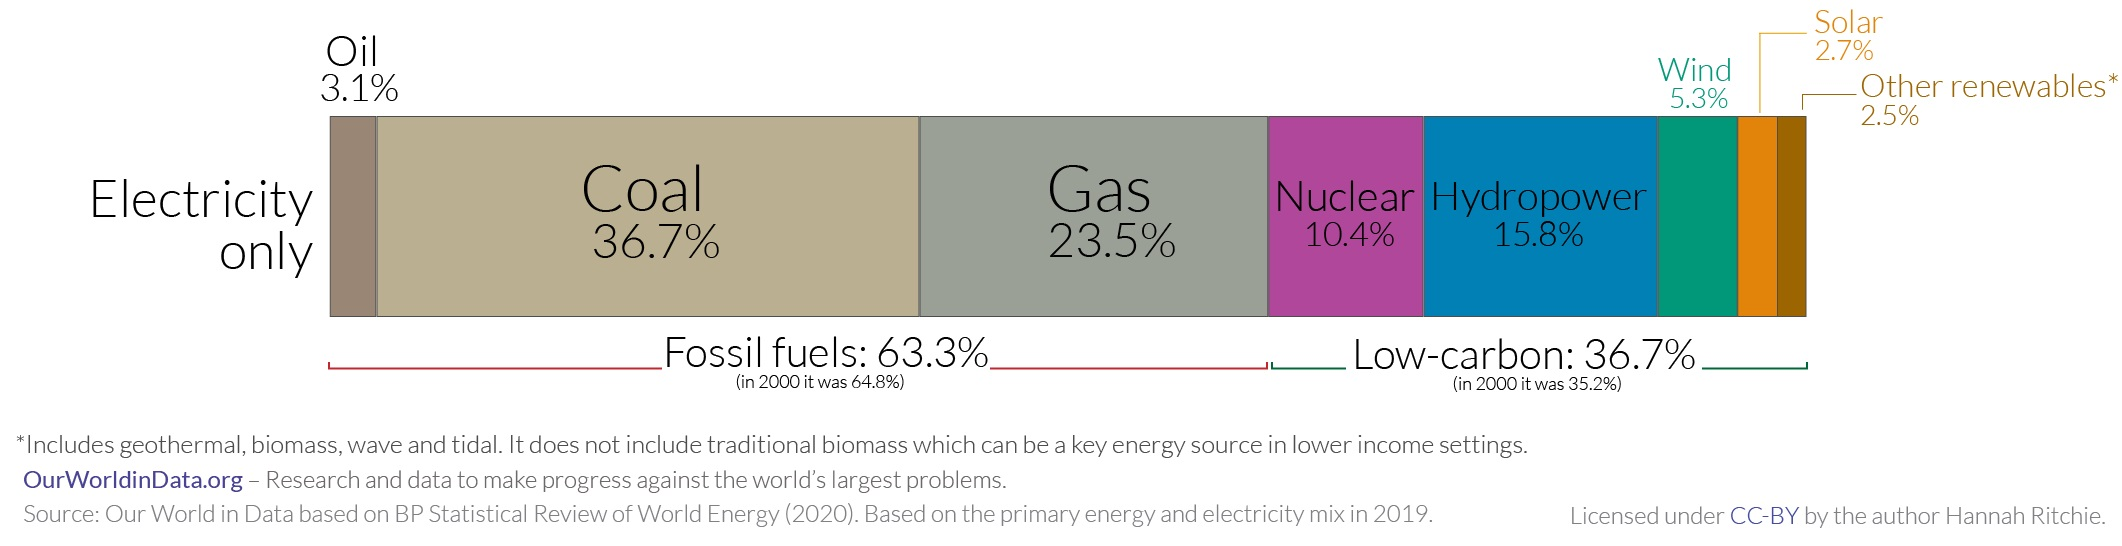
\includegraphics[width=1\textwidth]{img/Global_electricity_from_fossil_fuels.jpg}
  \caption{Global electricity production from fossil fuels\protect\footnotemark.}
  \label{fig:Global_electricity_from_fossil_fuels}
\end{figure}
\footnotetext{\url{https://ourworldindata.org/uploads/2020/08/Global-energy-vs.-electricity-breakdown-1536x812.png}}
\vspace{-10pt}

The consumption of electricity has risen due to the increased use of devices in various sectors such as home, entertainment, and more. Moreover, the number of smart devices (e;g.IoT Devices) is expected to grow more than twice by the end of this decade. By 2040, billions of IoT devices could contribute up to 14 percent of the world’s carbon emissions\footnote{\url{https://www.theguardian.com/environment/2017/dec/11/tsunami-of-data-could-consume-fifth-global-electricity-by-2025}}.

\vspace{-12pt}
\vspace{3em}
\begin{figure}[h]
  \centering
  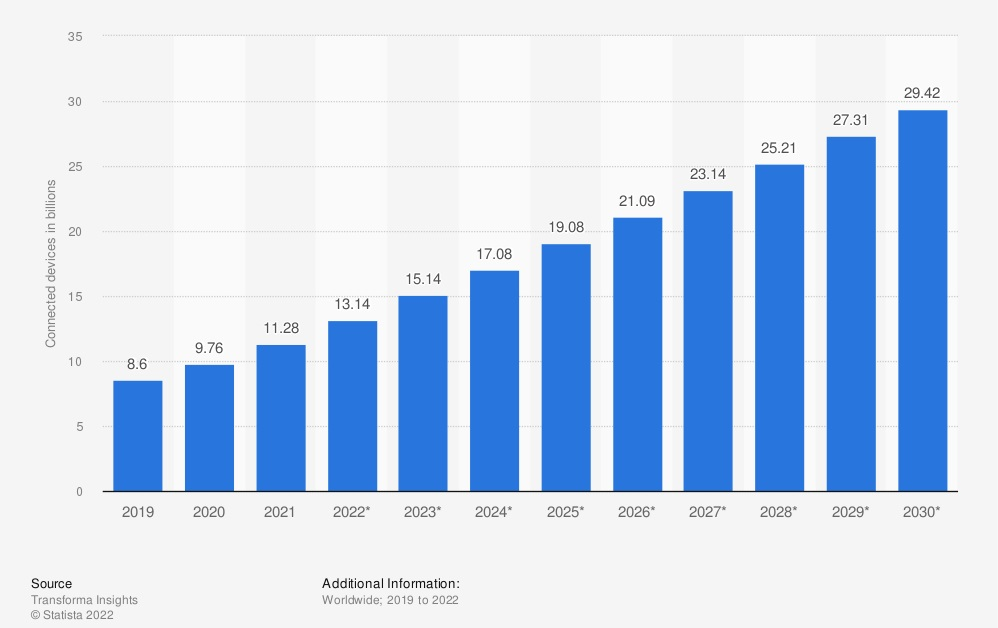
\includegraphics[width=.7\textwidth]{img/Number-of-iot-connected-devices-worldwide-2019-2021-with-forecasts-to-2030.jpg}
  \caption{Number of IOT connected devices worldwide (2019-2021) with forecasts to 2030.\protect\footnotemark}
  \label{fig:Number-of-iot-connected-devices-worldwide-2019-2021-with-forecasts-to-2030.jpg}
\end{figure}
\footnotetext{\url{https://www.statista.com/statistics/1183457/iot-connected-devices-worldwide/}}
\vspace{-15pt}

As the use of IoT devices becomes more widespread, energy consumption has become a major concern. Researchers are working on ways to make both hardware and software components of devices more energy-efficient. While software itself does not consume energy, its architecture, structure, and usage context can influence the energy consumption of hardware. By configuring software to be more energy-efficient, we can reduce energy consumption and carbon emissions, contributing to the preservation of our planet.\par


%\vspace{.5em}
%The increase in  CO\textsubscript{2} emissions leads to global warming and changes in climate and weather patterns, resulting in more floods, droughts, or intense rain, as well as more frequent and severe heat waves. The planet’s oceans and glaciers are also affected—oceans are warming and becoming more acidic, ice caps are melting, and sea level is rising. These changes present challenges to our society and our environment, including health risks from heat waves, worsening air and water quality, and the spread of certain diseases.


\vspace{.5em}
Software, gaming services on various devices, servers, networks infrastructure and data centers generate a significant amount of carbon dioxide emissions. The servers and data centers also need to use a huge amount of energy to maintain the temperature so that the machines can work more efficiently. According to a study by Abraham, every company, studio, and developer he gathered data on including Ubisoft, Nintendo, and Microsoft were all somewhere in the range of generating 1 to 5 tons of CO\textsubscript{2} per year\footnote{\url{https://www.polygon.com/features/22914488/video-games-climate-change-carbon-footprint}}. 

\begin{figure}[htbp]
  \centering
  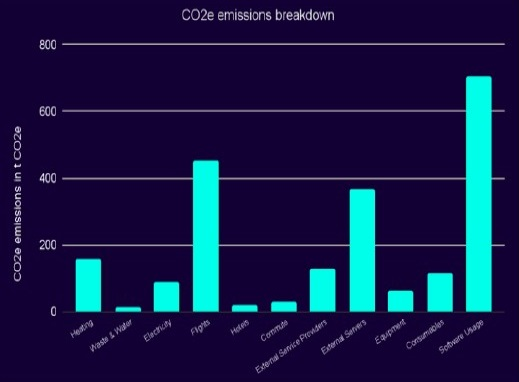
\includegraphics[width=.5\textwidth]{img/CO2_emission_each_level.jpg}
  \caption{CO\textsubscript{2}e emissions breakdown.\protect\footnotemark}
  \label{fig:CO2_emission_each_level}
\end{figure}
\footnotetext{\url{https://www.planetly.com/articles/what-tech-companies-can-do-to-reduce-and-avoid-emissions}}

\vspace{.5em}
To comprehend the energy consumption associated with software, the following examples are provided:
In 2019, researchers found that the energy used to keep the Bitcoin network running was more than the energy used by the whole country of Switzerland\footnote{\url{https://hbr.org/2020/09/how-green-is-your-software}}. Training a single neural network model today can emit as much carbon as five cars in their lifetimes\footnotemark[9]. Researchers trained an AI model to recognize different types of iris flowers. The model was 96.17\% accurate and used 964 joules of energy. To make the model 1.74\% more accurate, it needed 2,815 joules of energy. To make it just 0.08\% more accurate, it needed almost 4 times more energy than the first stage\footnotemark[9].

\vspace{.5em}
Energy consumption plays a pivotal role in contributing to global carbon dioxide emissions, making it crucial to address this issue in the context of software development. While modifying user behavior to reduce energy consumption can be challenging, there are opportunities to assist developers and other stakeholders in integrating energy efficiency considerations throughout the software development life cycle. For example: Puzzling out Software Sustainability \cite{DBLP:journals/suscom/CaleroP17}.

\vspace{.5em}
Energy efficiency is crucial in Cyber-Physical Social Systems (CPSS), which combine computing, physical processes, and social interactions. As these systems grow in complexity, they use more energy, impacting the environment. Making the software in CPSS more energy-efficient can cut down its overall energy use and reduce its carbon footprint. This not only helps the planet but also makes the system run better and be more resilient. The unique blend of tech and social elements in CPSS offers both challenges and opportunities for making it more energy-efficient. Thus, focusing on energy-smart software is key to fighting global climate change.

\vspace{-10pt}
\section{Problem Statement}
\label{sec:problem_statement}
The energy efficiency of software development is often overlooked by software developers, leading to suboptimal energy consumption in software applications. This lack of awareness and consideration for energy efficiency can be attributed to several factors:

\begin{itemize}
\vspace{-5pt}
\item Currently, there is a lack of direct energy awareness that enable software developers to measure and understand the energy consumption of their source code during the development phase. This absence hinders the ability to identify and address energy inefficiencies early on.
\vspace{-5pt}
\item Software developers generally lack sufficient knowledge and awareness about how to save energy by optimizing their source code. Without the necessary guidance and information, they may unknowingly contribute to excessive energy consumption in their software applications.
\end{itemize}

Due to its platform independence and strong security features, Java dominated the programming language landscape as the most popular choice from 2015 to 2020. Despite its decline in recent years, Java still holds a significant position as the fifth most popular programming language and continues to be extensively utilized in server environments\footnote{\url{https://insights.stackoverflow.com/survey/2020#most-popular-technologies}}. Though python is the most energy consuming Programming Language, it is also found by the researchers that Java also consumes more energy than C, C++. For example: Ranking programming languages by energy efficiency \cite{DBLP:journals/scp/PereiraCRRCFS21}. Given Java programming language's historical prominence, machine independence, security capabilities, and widespread adoption in server applications, we have selected Java as our primary focus for further research and development efforts.

\vspace{-10pt}
\section{Objectives}
\label{sec:Objectives}

In our research, we will undertake a thorough exploration of various tactics aimed at improving software energy efficiency. We will not only identify these tactics but also provide detailed insights into their implementation, highlighting practical ways to integrate them into the software development process. The main objective of this study is to explore tactics for enhancing software energy efficiency. From this objective we define 2 research questions:
\begin{itemize}
    \item RQ1: Which tactics help to improve Energy Efficiency?
    \item RQ2: How can we automatise the integration of tactics to reduce energy consumption?
    \begin{itemize}
    \item \small RQ2.1 Does the improvement of \textit{execution time} and  \textit{memory consumption} reduce energy consumption?
    \item \small RQ2.2 Could code refactoring integrate into GI? Which elements need to be extended in the Gin tool?
    \item \small RQ2.3: In which extent code refactoring genetically improve the software to reduce energy consumption?
  \end{itemize}
\end{itemize}

\vspace{-5pt}
In response to Research Question 1 (RQ1), we explore tactics for improving energy efficiency, primarily focusing on code refactoring. We explore code refactoring as our main tactic due to its significant impact on energy conservation. We will delve into various code refactoring methods, including state-of-the-art techniques. Our ultimate goal is to elucidate how this tactical approach contributes to enhancing the energy efficiency of software.\par

\vspace{.5em}
In RQ2, we focus on automating the integration of tactics to lower energy consumption. The approach involves using a genetic improvement, and as part of the research, a tool called GIN will be introduced. GIN is designed to improve existing software using search-based techniques. Three sub-questions have been identified: RQ2.1 aims to verify if improvements in response time and memory consumption(individually or together) can result in energy reduction. Experiments will be conducted using the GIN tool, with optimized versions compared to their original version using JoulerJX to assess energy impact. RQ2.2 investigates the feasibility of integrating code refactoring into Genetic Improvement (GI), identifying necessary extensions to the GIN tool. Finally, RQ2.3 explores the extent to which the integration of code refactoring can genetically enhance software to reduce energy consumption, testing its impact on energy efficiency.\par

\vspace{-10pt}
\section{Conclusion}

The efficient utilization of smart devices and the transition towards sustainable energy sources are crucial topics of global significance. It is essential for individuals and communities to remain cognizant of their electricity consumption and to promote energy efficiency. By raising awareness and making small changes in our daily lives, we can collectively contribute to reducing the strain on non-renewable resources and pave the way for a greener, more sustainable future.

\vspace{.5em}
The research comprised several distinct chapters. In the first chapter, the motivation behind the study, the objectives to be achieved, and the problem statement were discussed. In the second chapter, we delved into tactics for enhancing software energy efficiency, analyzed their respective benefits and limitations, and identified a tactic. Additionally, we emphasized the importance of energy consumption monitoring and selected \textit{JoularJX} as our primary tool for monitoring energy consumption in Java-based applications. The third chapter provided an in-depth literature review focusing on the themes of code refactoring and genetic improvement in software. Chapter four detailed a preliminary study aimed at understanding software energy consumption using the \textit{JoularJX} tool, illustrating its installation process and the initial experiments that were conducted using this tool. In Chapter five, we presented the results of our experiments, compared the energy consumption of the original and optimized programs using the \textit{Gin} tool, and discussed the implications for software energy efficiency. The sixth chapter was for the conclusion and discussions on future work.

